\documentclass[]{article}
\usepackage{lmodern}
\usepackage{amssymb,amsmath}
\usepackage{ifxetex,ifluatex}
\usepackage{fixltx2e} % provides \textsubscript
\ifnum 0\ifxetex 1\fi\ifluatex 1\fi=0 % if pdftex
  \usepackage[T1]{fontenc}
  \usepackage[utf8]{inputenc}
\else % if luatex or xelatex
  \ifxetex
    \usepackage{mathspec}
  \else
    \usepackage{fontspec}
  \fi
  \defaultfontfeatures{Ligatures=TeX,Scale=MatchLowercase}
\fi
% use upquote if available, for straight quotes in verbatim environments
\IfFileExists{upquote.sty}{\usepackage{upquote}}{}
% use microtype if available
\IfFileExists{microtype.sty}{%
\usepackage{microtype}
\UseMicrotypeSet[protrusion]{basicmath} % disable protrusion for tt fonts
}{}
\usepackage[margin=1in]{geometry}
\usepackage{hyperref}
\hypersetup{unicode=true,
            pdftitle={El Niño drives foreign fishing},
            pdfborder={0 0 0},
            breaklinks=true}
\urlstyle{same}  % don't use monospace font for urls
\usepackage{natbib}
\bibliographystyle{plainnat}
\usepackage{graphicx,grffile}
\makeatletter
\def\maxwidth{\ifdim\Gin@nat@width>\linewidth\linewidth\else\Gin@nat@width\fi}
\def\maxheight{\ifdim\Gin@nat@height>\textheight\textheight\else\Gin@nat@height\fi}
\makeatother
% Scale images if necessary, so that they will not overflow the page
% margins by default, and it is still possible to overwrite the defaults
% using explicit options in \includegraphics[width, height, ...]{}
\setkeys{Gin}{width=\maxwidth,height=\maxheight,keepaspectratio}
\IfFileExists{parskip.sty}{%
\usepackage{parskip}
}{% else
\setlength{\parindent}{0pt}
\setlength{\parskip}{6pt plus 2pt minus 1pt}
}
\setlength{\emergencystretch}{3em}  % prevent overfull lines
\providecommand{\tightlist}{%
  \setlength{\itemsep}{0pt}\setlength{\parskip}{0pt}}
\setcounter{secnumdepth}{0}
% Redefines (sub)paragraphs to behave more like sections
\ifx\paragraph\undefined\else
\let\oldparagraph\paragraph
\renewcommand{\paragraph}[1]{\oldparagraph{#1}\mbox{}}
\fi
\ifx\subparagraph\undefined\else
\let\oldsubparagraph\subparagraph
\renewcommand{\subparagraph}[1]{\oldsubparagraph{#1}\mbox{}}
\fi

%%% Use protect on footnotes to avoid problems with footnotes in titles
\let\rmarkdownfootnote\footnote%
\def\footnote{\protect\rmarkdownfootnote}

%%% Change title format to be more compact
\usepackage{titling}

% Create subtitle command for use in maketitle
\newcommand{\subtitle}[1]{
  \posttitle{
    \begin{center}\large#1\end{center}
    }
}

\setlength{\droptitle}{-2em}

  \title{El Niño drives foreign fishing}
    \pretitle{\vspace{\droptitle}\centering\huge}
  \posttitle{\par}
  \subtitle{Submission for AERE Sponsored and General Sessions (998 Words)}
  \author{Juan Carlos Villaseñor-Derbez\textsuperscript{a} Kimberly
Oremus\textsuperscript{b}}
    \preauthor{\centering\large\emph}
  \postauthor{\par}
      \predate{\centering\large\emph}
  \postdate{\par}
    \date{\textsuperscript{a}Bren School of Environmental Science \& Management,
University of California Santa Barbara. Email: juancarlos@ucsb.edu \textsuperscript{b}School of
Marine Science and Policy, University of Delaware. Email: oremus@udel.edu}

\usepackage{float}
\floatplacement{figure}{H}

\begin{document}
\maketitle

Warming oceans are causing marine taxa to redistribute poleward and to deeper waters \citep{pinsky_2013}. As species shift poleward, stocks are expected to move out of, into, and across Exclusive Economic Zones \citep{poloczanska_2013}, having major implications for fisheries management and livelihoods of these countries. This redistribution can also be caused by processes acting at a shorter timescale, like El Niño Southern Oscillation (ENSO). For example, Pacific Island Nations that are Parties to the Nauru Agreement (PNA) manage tuna stocks within their EEZs under a vessel-day scheme similar to a cap-and-trade regulation. La Niña and El Niño phases are associated with greater catches in the western and eastern boundaries of the PNA regions, respectively. As productivity shifts longitudinally, fishing permits and therefore allocation of fishing effort follow \citep{aqorau_2018}.

This problem has led to calls from the scientific community to generate institutions that can provide resilience to climate variation and prepare ocean governance for ``species on the move'' \citep{pinsky_2018}. However, the extent to which these short- and long-term shifts result in behavioral changes from resource users has not been explored or empirically estimated. In this paper we combine vessel-detection technology and empirical identification strategies to quantify the effect of climate variability (\emph{i.e.} ENSO) on foreign fishing behavior.

We use data from Global Fishing Watch (GFW; \href{www.globalfishingwatch.org}{globalfishingwatch.org}) to quantify the effect that ENSO has on foreign fishing. The vessel-detection database is a panel of fishing vessels for which we observe flag, gear, position (\emph{i.e.} latitude, longitude) and duration of fishing events (hours) from 2012 to present \citep{kroodsma_2018}. Our dataset contains information for a total of 26000 vessels from 13 countries (Fig \ref{fig:gfw}). We define foreign fishing as any fishing event in which a vessel's reported flag does not match the jurisdiction of the Exclusive Economic Zone in which fishing takes place, and restrict our analyses to two main fishing gears: longliners and purse seiners. Longliners use a mother line with hundreds to thousands of baited hooks every few meters. Purse seiners use nets to enclose large schools of fish. Both methods are largely used for commercially important species, like Tuna and Swordfish.

Temperature is one of the main environmental variables that drives species redistribution \citep{pinsky_2013}. However, climate indices can be useful summaries of systemic, environmental variation \citep{meng_2016}. We use a time series of ENSO anomalies (NINO3; Fig 2) and combine it with a spatially-explicit time series of global Sea Surface Temperature (SST) to identify regions where changes in NINO3 correspond to changes in SST. This approach has been previously used to identify ``ENSO-teleconnected regions'' \citep{hsiang_2011}. This allows us to identify regions where fishing effort is likely to be affected by changes between negative and positive ENSO phases (Fig. 3).

Our empirical strategy uses a difference-in-differences approach. We estimate the effects of ENSO on Foreign Fishing by comparing the effects between regions impacted by ENSO and regions not impacted by ENSO:

\[
log(FF_{rgct}) = \beta ENSO_{t} \times \mathbb{I}_{Lat, Lon \epsilon r} + \gamma ENSO_{t} + \xi \mathbb{I}_{Lat, Lon \epsilon r} + \theta_{g} + \phi_{t} + \lambda_{c} + \epsilon_{rgct}
\]

\clearpage

\(FF_{gct}\) represents the foreign fishing variable of interest by gear, country and year. In the main specification, we use an inverse hyperbolic sine of foreign fishing, which approximates a log transform of FF\footnote{\(ln(FF + \sqrt{1 + FF^2}) \rightarrow ln(2L)\)}, to transform zeroes in our data \cite{Burbidge:1988, Card:2017}. \(\alpha\) is a constant and \(\beta\) captures the linear effect of ENSO on affected regions compared to regions unaffected by ENSO. The treatment is ENSO and it is interacted with a dummy, \(\mathbb{I}_{Lat, Lon \epsilon r}\), that equals 1 for regions in the ENSO-affected region and 0 for counties in unaffected-ENSO regions. \(\gamma\) is the average effect of ENSO over both the treated and untreated regions and \(\xi\) is the average effect of being in the treatment region vs.~not being in the treatment region. \(\theta_{g}\) are gear fixed effects, \(\phi_{t}\) are monthly fixed effects and \(\lambda_{c}\) are country (flag) fixed effects.

Our results suggest that positive ENSO phases lead to an increase in foreign fishing hours. The result is robust across a set of specifications and to both measures of foreign fishing (\emph{i.e.} hours and their hyperbolic transformation; Table \ref{tab:ff_reg}). The base model shows that, on average, a one-unit increase in the NINO3 index leads to a 2\% increase in foreign fishing hours per month for all vessels (\emph{i.e.} vessels in treated and untreated regions). At the same time, we find a positive interaction effect of 4\% additional foreign fishing hours per unit increase in NINO3 index for vessels in ENSO-affected regions. The NINO3 index can often vary by more than two-and-a-half units on either direction (see Fig. 2), which would translate as a 10\% increase in foreign fishing. We also run this on a subsample of boats that fish in both the treated and untreated region.

Our results also suggest that the change in foreign fishing hours is greater for longliners than for purse seiners. This may be related to how adaptive these gears are, or to the restriction that a variable climate induces on each gear. For example, positive ENSO phases are known to increase thermocline depth causing species such as tuna to swim deeper in search of cooler temperatures. This facilitates escapement of tuna in shallow purse seine nets and increases the proportion of null sets\footnote{Null sets are described as events where purse seiners cast their nets around tuna, but these manage to escape under the net before the set is completed.} in Mexican tuna purse seiners \citep{dreyfusleon_2015}. This may also be due to the fact that longliners are harder to regulate since they are the most abundant vessels and are highly mobile \citep{sala_2018,ortuocrespo_2018}.

Our results suggest that positive ENSO phases lead to an increase in foreign fishing hours. This quantitative evidence linking climate and fishing behavior has important implications for fisheries management, economics of climate projections and adaptation of this sector.

\clearpage

\hypertarget{figures-and-tables}{%
\section{Figures and tables}\label{figures-and-tables}}

\begin{figure}
\centering
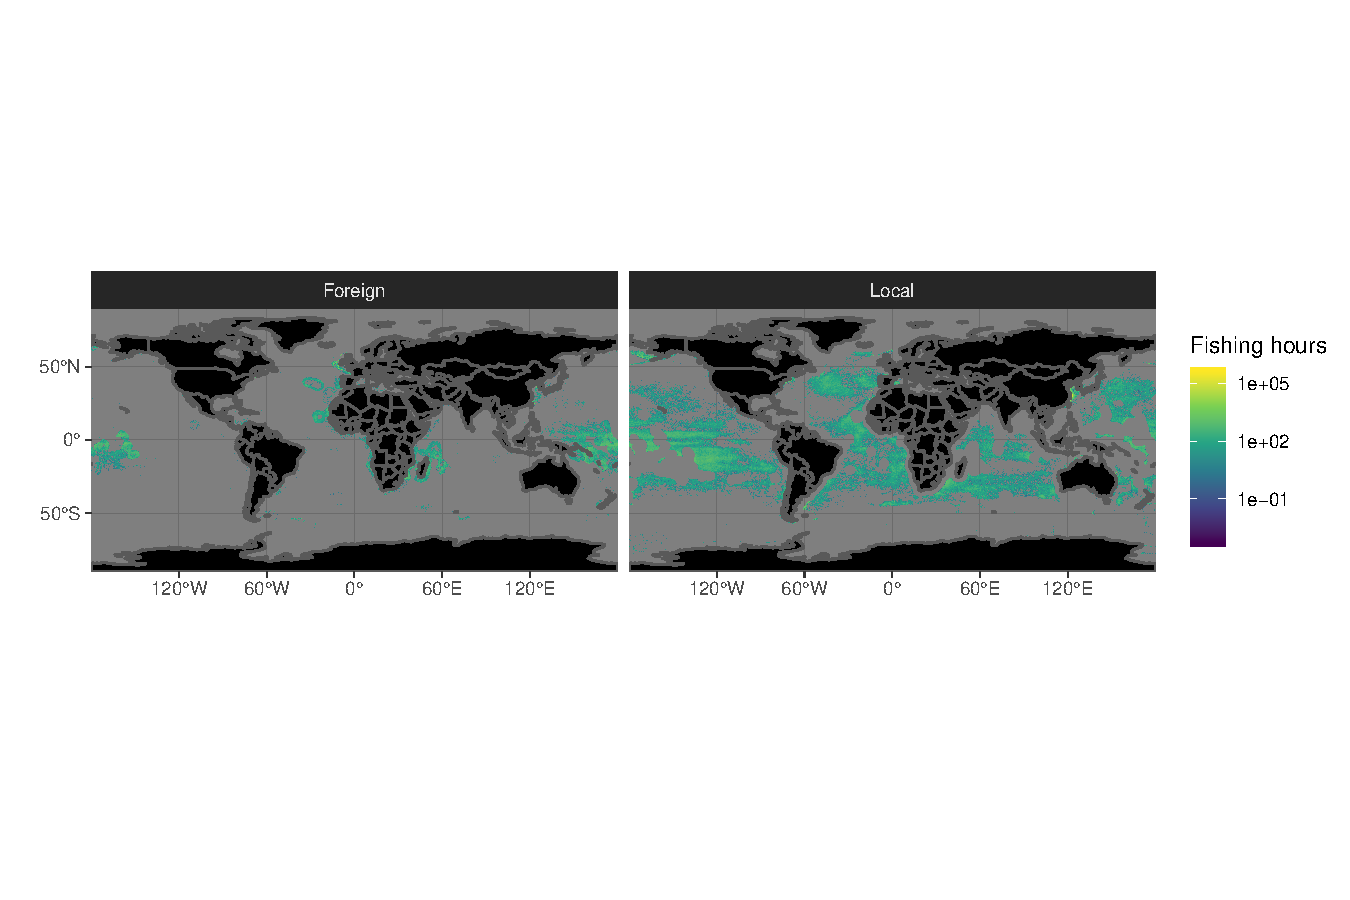
\includegraphics{img/GFW_raster.pdf}
\caption{\label{fig:gfw} Local and foreign fishing effort from 2012 - 2017 (hours).}
\end{figure}

\begin{figure}
\centering
\includegraphics{img/AERE_nino3.pdf}
\caption{Timeseries of NINO3 index (detrended). The gray shaded area  higlights the period with vessel data coverage}
\end{figure}

\begin{figure}
\centering
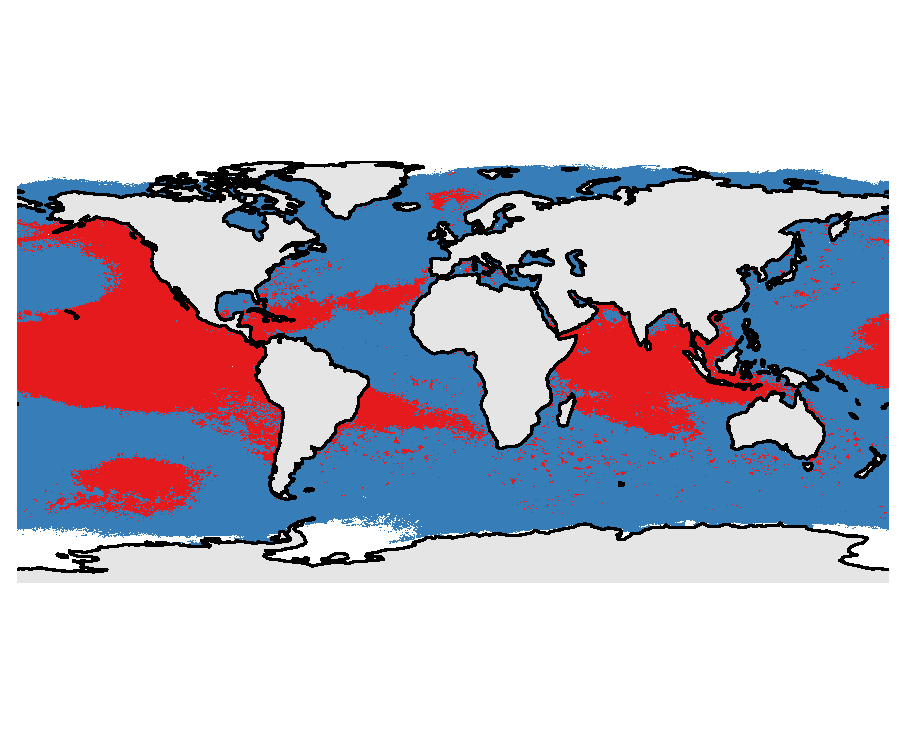
\includegraphics{img/teleconnected_3months.pdf}
\caption{\label{fig:teleconnections} ENSO-Teleconnected marine regions.
Red and blue indicate the when where SST showed a positive (r
\textgreater{} 0) and significant (p \textless{} 0.1) correlation with
NINO3 index for at least 3 months. White areas represent areas where SST
data is no available.}
\end{figure}

\clearpage

\begin{table}[!htbp] \centering 
  \caption{\label{tab:ff_reg}Effect of NINO3.4 anomally index on foreign fishing for purse seiners (1-3) and longliners(4-6).} 
  \label{} 
\begin{tabular}{@{\extracolsep{5pt}}lcccccc} 
\\[-1.8ex]\hline 
\hline \\[-1.8ex] 
 & \multicolumn{6}{c}{\textit{Dependent variable:}} \\ 
\cline{2-7} 
\\[-1.8ex] & \multicolumn{6}{c}{Monthly foreign fishing hours} \\ 
\\[-1.8ex] & (1) & (2) & (3) & (4) & (5) & (6)\\ 
\hline \\[-1.8ex] 
 nino34anom & $-$0.010$^{***}$ & $-$0.011$^{***}$ & $-$0.014$^{***}$ & 0.013$^{***}$ & 0.015$^{***}$ & 0.015$^{***}$ \\ 
  & (0.001) & (0.001) & (0.001) & (0.001) & (0.001) & (0.001) \\ 
  & & & & & & \\ 
 treated & $-$0.176$^{***}$ & $-$0.170$^{***}$ & 0.031$^{***}$ & $-$0.021$^{***}$ & $-$0.016$^{***}$ & $-$0.086$^{***}$ \\ 
  & (0.001) & (0.001) & (0.003) & (0.001) & (0.001) & (0.002) \\ 
  & & & & & & \\ 
 nino34anom:treated & 0.069$^{***}$ & 0.070$^{***}$ & 0.077$^{***}$ & 0.031$^{***}$ & 0.027$^{***}$ & 0.031$^{***}$ \\ 
  & (0.001) & (0.001) & (0.001) & (0.002) & (0.002) & (0.002) \\ 
  & & & & & & \\ 
 Constant & 1.177$^{***}$ & 1.120$^{***}$ & 2.132$^{***}$ & 1.318$^{***}$ & 1.297$^{***}$ & 2.303$^{***}$ \\ 
  & (0.001) & (0.002) & (0.042) & (0.001) & (0.002) & (0.113) \\ 
  & & & & & & \\ 
\hline \\[-1.8ex] 
Month FE & No & Yes & Yes & No & Yes & Yes \\ 
Country FE & No & No & Yes & No & No & Yes \\ 
Observations & 3,819,575 & 3,819,575 & 3,819,575 & 5,086,606 & 5,086,606 & 5,086,606 \\ 
R$^{2}$ & 0.005 & 0.006 & 0.023 & 0.0003 & 0.002 & 0.026 \\ 
\hline 
\hline \\[-1.8ex] 
\textit{Note:}  & \multicolumn{6}{r}{$^{*}$p$<$0.1; $^{**}$p$<$0.05; $^{***}$p$<$0.01} \\ 
\end{tabular} 
\end{table} 

\begin{table}[!htbp] \centering 
  \caption{\label{tab:ff_reg}Effect of NINO3.4 anomally index on foreign fishing for purse seiners (1-3) and longliners(4-6).} 
  \label{} 
\begin{tabular}{@{\extracolsep{5pt}} c} 
\\[-1.8ex]\hline 
\hline \\[-1.8ex] 
TRUE \\ 
\hline \\[-1.8ex] 
\end{tabular} 
\end{table} 

\clearpage

\renewcommand\refname{References}
\bibliography{references}


\end{document}
